\clearpage
\section{Automatyzacja pracy z submodułami}
\label{sec:gitio}

Ninejszy rozdział jest poświęcony obsługi wielopoziomowej struktury opartej o \emph{git submodules} obecnej w projekcie GGSS. Przedstawione zostaną plusy oraz minusy zastosowanego w trakcie pracy inżynierskiej rozwiązania. Omówiona zostanie przygotowana przez autorów infrastruktura mająca na celu ułatwienie pracy z submodułami. Dodatkowo krótko zostanie opisane przygotowane \emph{how-to} oraz praktyki które powinno się stosować pracując z taką architekturą.

\subsection{Wprowadzenie do problematyki}

W trakcie pracy inżynierskiej, a konkretnie migracji całego projektu GGSS do systemu kontroli wersji \emph{git} zdecydowano się na wykorzystanie technologii \emph{git submodules}. Ze względu na nacisk na zwiększenie modularyzacji projektu technologia ta idealnie wpasowywała się w docelową architekurę. Zasada działania submodułów jest bardzo zbliżona do dowiązań symbolicznych stosowanych między innymi w systemach UNIX. Zamiast wskazywać na ścieżkę do folderu na lokalnym systemie submoduł wskazuje na ścieżkę do konkretnej wersji repozytorium na zewnętrznym serwerze od którego zależy nasz moduł. Rysunek \ref{fig:submodules_links} przedstawia zasadę działania submodułów oraz wpływ wersjonowania na tenże mechanizm. Wykorzystanie submodułów pozwala na w pełni odseparowaną pracę nad wybranym komponentem systemu. Nie potrzebujemy pobierać żadnych dodatkowych plików, czy też zależności w celu zmienienia kodu źródłowego. Rozwiązanie to pozwala też na skorzystanie z bardzo szybkiej inicjalizacji całego projektu jedną komendą, co zostało przedstawione w listingu \ref{lst:initialize}.

\begin{figure}[H]
    \centering
    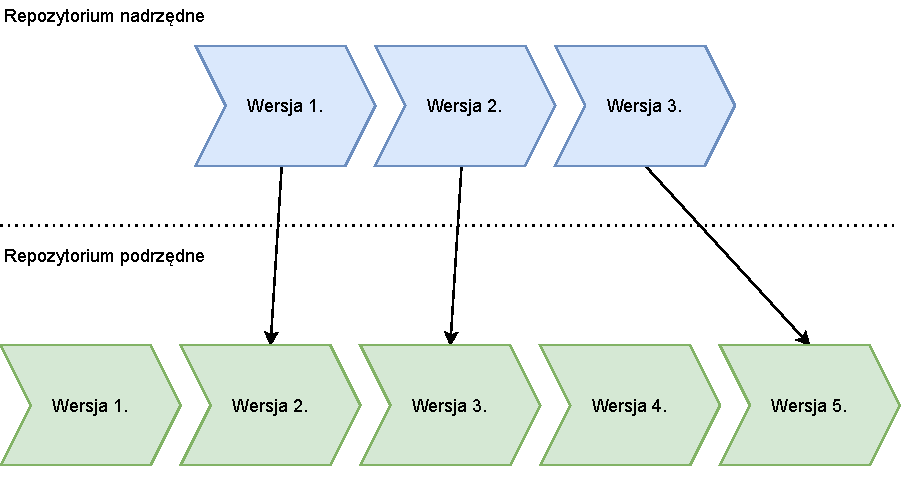
\includegraphics[width=0.9\textwidth]{components/infra/gitio_submodules_res/submodule_links}
    \caption{Zasada działania submodułów.}
    \label{fig:submodules_links}
\end{figure}

\begin{lstlisting}[language=c++, caption={Inicjalizacja pełnej sturktury projektu jedną komendą.}, label={lst:initialize}]
root@host:/# git clone ssh://git@gitlab.cern.ch:7999/atlas-trt-dcs-ggss/ggss-all.git && cd ggss-all && git submodule update --init --recursive
Cloning into '/CERN/ggss-all/ggss-dim-cs'...
Cloning into '/CERN/ggss-all/ggss-driver'...
Cloning into '/CERN/ggss-all/ggss-oper'...
Cloning into '/CERN/ggss-all/ggss-runner'...
Cloning into '/CERN/ggss-all/ggss-spector'...
Cloning into '/CERN/ggss-all/mca-n957'...
Cloning into '/CERN/ggss-all/ggss-dim-cs/external-dim-lib'...
Cloning into '/CERN/ggss-all/ggss-dim-cs/ggss-misc'...
Cloning into '/CERN/ggss-all/ggss-driver/external-n957-lib'...
Cloning into '/CERN/ggss-all/ggss-driver/ggss-misc'...
...(13 lines truncated)
\end{lstlisting}


\subsection{Motywacja do wprowadzenia zmian}

Pomimo wielu aspektów \emph{git submodules}, które bardzo dobrze wpasowały się w, kreowaną przez autorów w trakcie pracy inżynierskiej, sturkturę technologia ta posiada też swoje minusy. Pierwszy znaczącym problemem napotkanym w trakcie pracy z submodułami było nietypowe zachowanie repozytoriów w trakcie ich inicjalizacji, a konkretnie automatyczne odłączanie ich od głównej gałęzi. Co więcej praca z submodułami wymaga od programisty zwiększonej czujności oraz stosowania dodatkowych zasad, ponieważ więcej jest miejsc na pomyłkę, co może doprowadzić do niepoprawnego działania wykorzystanych narzędzi. Kolejnym problemem napotkanym w trakcie pracy z submodułami jest czasochłonność niektórych operacji, w szczególności aktualizacji repozytorium na samym dole ``drzewa zależności``. Zmiana taka wymaga ręcznej aktualizacji po kolei każdego z repozytorium, aż do samej góry tejże skruktury co przedstawia rysunek \ref {fig:submodules_update}. Każda z aktualizacji przedstawiona na wyżej wymieionym rysunku, to tak na prawdę cztery lub więcej akcji do których wliczają się: aktualizacja repozytorium podrzędnego, dodanie wszystkich zmian do rejestru odpowiedzialnego za ich śledzenie, utworzenie nowej wersji repozytorium, opublikowanie nowej wersji na zewnętrznym serwerze.



\clearpage
\begin{figure}[H]
    \centering
    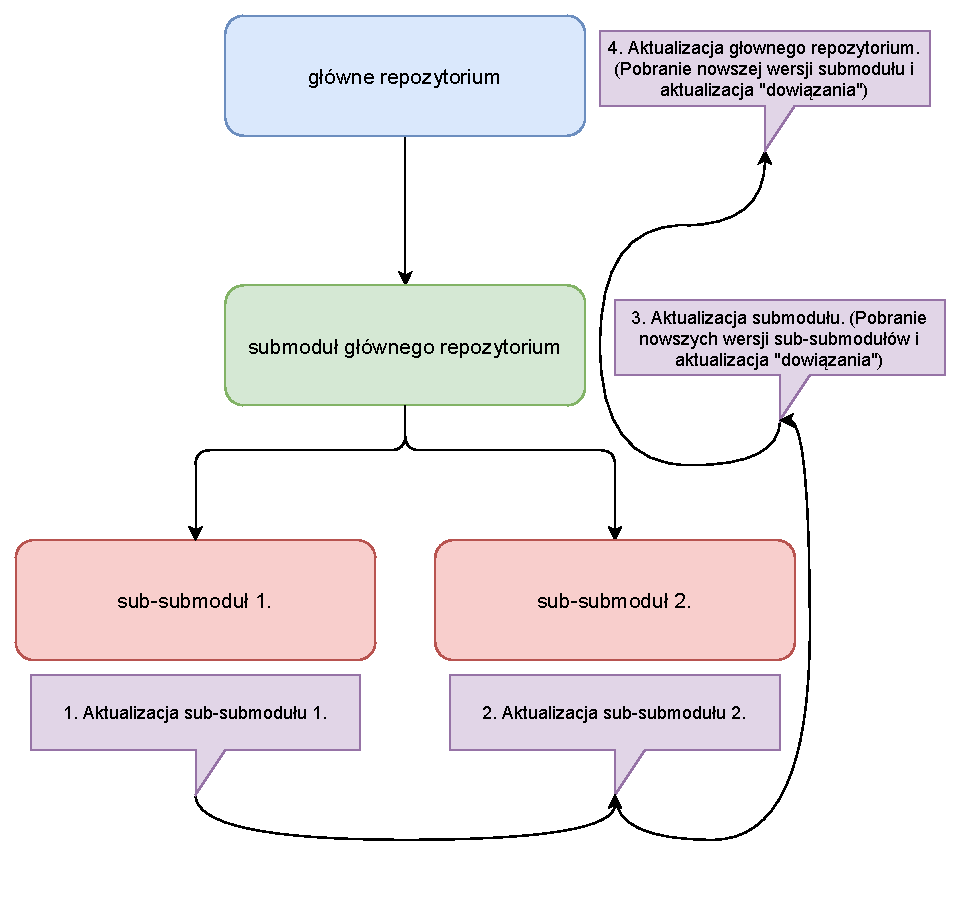
\includegraphics[width=0.9\textwidth]{components/infra/gitio_submodules_res/submodules_update}
    \caption{Przykładowa architektura oparta o submoduły z krokami jakie należy podjąć, aby wprowadzić zmiany na ``najniższym`` poziomie.}
    \label{fig:submodules_update}
\end{figure}


\subsection{Automatyzacja z użyciem GITIO}

Problemem, którego rozwiązanie pochłonęło najwięcej czasu i wymagało największego wkładu pracy przez autorów było monotonne, wielokrokowie wprowadzanie zmian do projektu, szczególnie u dołu struktury zależności. W celu rozwiązanie tego problemu przygotowano aplikacje \emph{gitio} z wykorzystaniem języka \emph{Python}. Ze względu na to, że metadane technologii \emph{git} są bardzo złożone, a opanowanie zasad węwnętrznego działania tejże technologii wymagałoby bardzo dużo czasu skorzystano z dedykowanej, do tej technologii, bilbioteki napisanej również w języku \emph{Python}.

Zasada działania aplikacji jest dosyć prosta, natomiast znacząco ułatwia działania z wielopoziomową strukturą opartą o \emph{git submodules}. Argumenty wejściowe jako przyjmuje \emph{gitio} to:
\begin{itemize}
    \item \lstinline{-h, --help} - pozwala na wyświetlnie informacji o przeznaczeniu programu oraz przyjmowanych argumentach wraz z krótkim opisem
    \item \lstinline{-p PATH, --path PATH} -
    \item \lstinline{-b BIN, --bin BIN} -
\end{itemize}

\subsection{Dokumentacja sposobu pracy z submodułami}

